\documentclass[border=20pt]{standalone}
%\usetikzlibrary{shapes.multipart,chains, positioning}

\usepackage{tikz}
\usetikzlibrary{calc,shapes.multipart,chains,arrows,positioning}

\tikzset{
myListFeader/.style={
	rectangle,draw=red!50,fill=red!20,thick,
	inner sep=0pt,minimum size=8mm
}
, myNull/.style={
	draw, rectangle,minimum size=2mm, fill=orange!80,
	inner sep=0pt, text=black,
	path picture = {
		\draw[black]
		(path picture bounding box.north west) -- (path picture bounding box.south east)
		(path picture bounding box.south west) -- (path picture bounding box.north east);
	}
}
%, myNode/.style={
%	rectangle,draw=blue!50,fill=blue!20,thick,
%	inner sep=0pt,minimum size=6mm
%}
, myNode/.style={
%	very thick, 
	thick, 
	rectangle split,
	rectangle split parts=3, draw,
	rectangle split horizontal, minimum size=6mm,
	rectangle split part fill={blue!20, white!20, red!20},
	inner sep=0pt, text=black
 }
% link
, myListF/.style={->,color=red!50,bend left=45,very thick}
, myListB/.style={->,color=red!50,bend right=45,very thick}
, myNext/.style={*->,color=red,bend left=45,thick}
%, myNextNull/.style={*->,color=red,bend left=45,thick}
, myPrev/.style={*->,color=blue,bend left=45,thick}
, myPrevNull/.style={*->,color=blue,bend right=45,thick}
}

\begin{document}


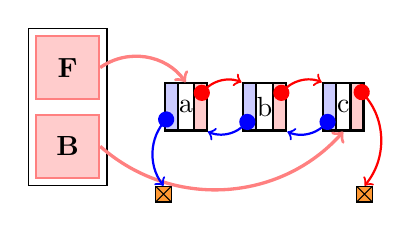
\begin{tikzpicture}
	% nodes
	\node[myNode] (A) at ( 0,0)  {\nodepart{second} a};
	\node[myNode] (B) at ( 1,0)  {\nodepart{second} b};
%	\node[myNode] (B) [right=of A]  {b};
	\node[myNode] (C) at ( 2,0)  {\nodepart{second} c};
	% null
	\node[myNull] (MyNullPrev)  [below=of A.west] {};
	\node[myNull] (MyNullNext)  [below=of C.east] {};
	% linked list node
	\draw (-2,1) rectangle (-1,-1);
	\node[myListFeader] (Front) at ( -1.5,0.5)  {\textbf{F}};
	\node[myListFeader] (Back) at ( -1.5,-0.5)  {\textbf{B}};
	\draw [myListF] (Front.east) to (A.north);
	\draw [myListB] (Back.east) to (C.south);
	
	% links
	\draw [myNext] ($(A.three) + (0.05, 0.16)$) to (B.north west);
	\draw [myPrevNull] ($(A.one)+ (0.1, -0.02)$) to (MyNullPrev.north);

	\draw [myNext] ($(B.three) + (0.05, 0.16)$) to (C.north west);
	\draw [myPrev] ($(B.one)+ (0.1, -0.02)$) to (A.south east);

%	\draw [myNextNull] ($(C.three) + (0.05, 0.33)$) to (MyNullNext.north);
	\draw [myNext] ($(C.three) + (0.05, 0.33)$) to (MyNullNext.north);
	\draw [myPrev] ($(C.one)+ (0.1, -0.02)$t) to (B.south east);
\end{tikzpicture}

\end{document}